\chapter{Marco Te\'orico}
  En este cap\'itulo se introducir\'a al lector en el framework \fud \ y en los conceptos b\'asicos de biolog\'ia para un mayor entendimiento de la
  aplicaci\'on implementada como parte de este trabajo final.

  \section{El Framework \fud}
    Computar grandes conjuntos de datos es una parte importante de las ciencias de la computaci\'on, mucha informaci\'on importante es inherentemente
    complicada de comprimir y, adem\'as, los recursos para procesar estos conjuntos de datos son usualmente costosos. Las organizaciones sin fines de
    lucro, las instituciones educativas y similares deben encontrar otros caminos para administrar sus requerimientos de procesamientos mientras
    mantienen sus costos lo m\'as bajo posible. Existen muchas herramientas para lograr una forma de computaci\'on distribuida en bajo costo.

    \fud \ (del acr\'onimo \textbf{F}uDePAN \textbf{u}biquitous \textbf{D}istribution) consiste en el dise\~no e implementaci\'on de un framework
    abstracto para implementar algoritmos distribuidos independientes de las herramientas antes mencionadas, de los sistemas de comunicaci\'on 
    subyacentes o alg\'un otro problema espec\'ifico.

    Este framework es un sistema separado en las capas de \textit{aplicaci\'on}, 
    \textit{administraci\'on} y \textit{distribuci\'on} combinando los conceptos de cliente-servidor y Divide \& Conquer. Tanto el cliente como el
    servidor se encuentran organizados en estos tres niveles (muy) separados, cada uno de ellos con una \'unica responsabilidad bien definida.
    \begin{figure}[H] \hspace{.60cm}
      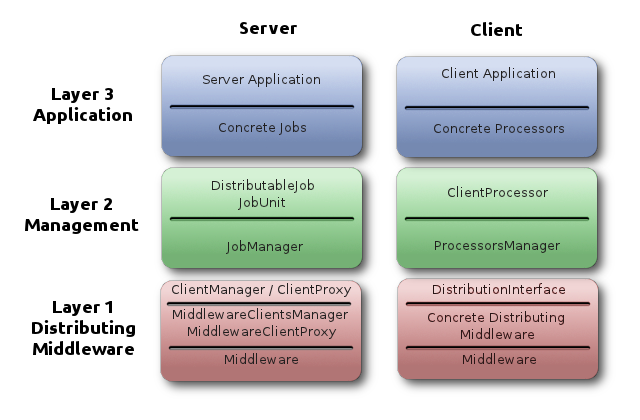
\includegraphics[scale=.51]{images/AbstractLayers.png}
      \caption{Vista abstracta de las capas en una instancia de uso de \fud} \label{disenioFud}
    \end{figure}
    La comunicaci\'on entre los diferentes niveles se encuentra estrictamente limitada, es decir, por cada nivel existe un \'unico punto de comunicaci\'on 
    ya sea para comunicarse con la capa superior o con la inferior siguiendo el enfoque OSI para redes.
    
    A continuaci\'on, muy brevemente, se explican cada una de las capas:
    \subsection{Application Layer (L3)}
    Este nivel provee los componentes que contienen todos los aspectos del dominio del problema. Estos aspectos incluyen todas las definiciones de los
    datos usados y su manipulaci\'on correspondiente, como as\'i tambi\'en todos los algoritmos relevantes para la soluci\'on al problema en general. Se debe
    tener en cuenta que bajo ninguna circunstancia esta capa pertenecer\'a a \fud \ pero su presencia es de ayuda para mostrar el uso del framework.

    \subsection{Job Management Layer (L2)}
    La responsabilidad de esta capa es manejar los trabajos que se desean distribuir como as\'i tambi\'en generar las unidades de trabajo que ser\'an
    entregadas a los clientes para su procesamiento. Estas unidades de trabajo llegan a su cliente correspondiente gracias a la capa m\'as baja, 
    encargada de la distribuci\'on. Una vez finalizado el procesamiento, es el nivel 2 quien informa que todo ha terminado y otorga los resultados a la capa superior.
  \newpage
    \subsection{Distributing Middleware Layer (L1)}
    A partir de esta vista abstracta del dise\~no, se debe notar que L1 solo constituye un esquema de administraci\'on de clientes en particular. Tal y
    como se observa en la figura \ref{disenioFud}, en ambos lados las partes fijas son las intarfaces del middleware, mientras que las
    implementaciones concretas son las partes variables (por ejemplo, BOINC o MPI).

    Notar que si se toma al proyecto \fud \ por separado, el mismo constituye una biblioteca que esta parcialmente implementada siempre y cuando el
    middleware de distribuci\'on est\'andar (boost::asio) sea removido. Esto lleva a que se pueden obtener diferentes sabores de la biblioteca \fud \
    con s\'olo reemplazar la capa de distribuci\'on (L1) por alguna otra. Por ejemplo, se podr\'ia utilizar MPI
    \footnote{\url{http://www.mcs.anl.gov/research/projects/mpi/}}, recomendado para clusters locales donde sus computadoras disponen de una 
    interconexi\'on veloz. Otra alternativa podr\'ia ser BOINC\footnote{\url{http://boinc.berkeley.edu/}} que posee una riqueza extrema en procesamiento,
    pero \'esta es llevada a cabo pagando el precio de la comunicaci\'on a trav\'es de Internet (la cual es bastante m\'as baja en velocidad con 
    respecto a otras configuraciones como Ethernet, infiniband, etc.). Estas diferentes implementaciones de la capa 1 deben ser intercambiables,
    es decir, uno puede variar entre ellas y el problema debe continuar siendo solucionable correctamente.

  \section{RNA Folding Free Energy}
  Como parte de esta tesis se implement\'o una aplicaci\'on de gran inter\'es para la fundaci\'on \fudepan \footnote{http://www.fudepan.org.ar/}. La descripci\'on
  e implementaci\'on de la misma se encuentra en el cap\'itulo \ref{RNAFFE_chapter}, en esta secci\'on presentamos los conceptos b\'asicos necesarios para comprender
  con mayor detalle la aplicaci\'on.

  \subsection{Organismos, Mol\'eculas y C\'elulas}
  \subsubsection{Organismos}
  Conjunto de biomol\'eculas org\'anicas e inorg\'anicas organizadas de manera especifica para cumplir determinadas funciones e interactuar con el medio en que se encuentran.
  
  \subsubsection{Mol\'eculas  Org\'anicas}
  Hay dos tipos de mol\'eculas org\'anicas b\'asicas:

  \begin{itemize}
    \item \emph{Nucle\'otidos}:
      Peque\~nas mol\'eculas constituyentes de macromol\'eculas de mayor complejidad. Los 5 tipos de nucle\'otidos m\'as importantes son:
      \begin{enumerate}
        \item Adenina (A) compone el ADN y el ARN.
        \item Guanina (G) compone el ADN y el ARN.
        \item Timina (T) compone el ADN.
        \item Citosina (C) compone el ADN y el ARN.
        \item Uracilo (U) compone el ARN.
      \end{enumerate}


    \item \emph{Amino\'acidos}:
      Son mol\'eculas que conforman las prote\'inas y son esenciales para la vida. A continuaci\'on se muestra una tabla conteniendo todos los amino\'acidos 
      y sus abreviaciones.
      \begin{center}
        \begin{tabular}{|ccc|}
          \hline Nombre & Ab. 3 letras & Ab. 1 Letra \\ 
          \hline Alanine & Ala & A \\ 
          \hline Arginine & Arg & R \\ 
          \hline Asparagine & Asn & N \\ 
          \hline Aspartic acid & Asp & D \\ 
          \hline Cytesine & Cys & C \\ 
          \hline Glutamic acid & Glu & E \\ 
          \hline Glutamine & Gln & Q \\ 
          \hline Glycine & Gly & G \\ 
          \hline Histidine & His & H \\ 
          \hline Isoleucine & Ile & I \\ 	
          \hline Leucine & Leu & L \\ 
          \hline Lysine & Lys & K \\ 
          \hline Methionine & Met & M \\ 
          \hline Phenylalanine & Phe & F \\ 
          \hline Proline & Pro & P \\ 
          \hline Serine & Ser & S \\ 
          \hline Threonine & Thr & T \\ 
          \hline Tryptophan & Trp & W \\ 
          \hline Tyrosine & Tyr & Y \\ 
          \hline Valine & Val & V \\ 
          \hline 
        \end{tabular} 
      \end{center}
  \end{itemize}


  \subsubsection{Macromol\'eculas}
  Son estructuras biol\'ogicas conformadas por un determinado n\'umero de mol\'eculas org\'anicas. Hay cuatro tipos de macromol\'eculas, \'Acidos Nucleicos, Prote\'inas, 
  Gl\'ucidos y L\'ipidos. S\'olo explicaremos las primeras dos ya que son las \'unicas relevantes para la aplicaci\'on:
  \begin{itemize}
    \item \emph{\'Acidos Nucleicos}: Est\'an conformados por secuencias de nucle\'otidos espec\'ificas, que son utilizadas por todos los organismos para almacenar su informaci\'on gen\'etica. La misma, est\'a codificada mediante sucesivos codones, los cuales est\'an conformados por tripletes de nucle\'otidos que codifican un amino\'acido. Dos de los \'acidos nucleicos m\'as importantes son:
      \begin{enumerate}
        \item \textbf{ADN (\'Acido Desoxirribonucleico)}: Contiene la informaci\'on gen\'etica para el desarrollo y el funcionamiento de los organismos vivos
	  y de algunos virus, la cual se hereda de generaci\'on en generaci\'on. Est\'a formado por una doble cadena de nucle\'otidos, en la que las dos hebras est\'an unidas a trav\'es de las bases complementarias, seg\'un el modelo propuesto por Watson y Crick en 1953.
        \item \textbf{ARN (\'Acido Ribonucleico)}: Consiste en una hebra de cadena simple, la cual usualmente es trascripta a partir de una porci\'on de ADN y se utiliza posteriormente en la c\'elula para la s\'intesis de prote\'inas. Algunos virus poseen ARN como \'unico material gen\'etico cuya monohebra puede plegarse, dando lugar a lo que se conoce como estructura secundaria, la cual se analizar\'a m\'as adelante.
      \end{enumerate}

    \item \emph{Prote\'inas:}
      Est\'an formadas por secuencias de amino\'acidos espec\'ificas, que adoptan una conformaci\'on tridimensional determinada debido a las interacciones electrost\'aticas existentes entre los residuos de sus amino\'acidos constituyentes. Este arreglo tridimensional la habilita para realizar una funci\'on en particular.
  \end{itemize}

  %\begin{figure}[h!]
  %\centering
  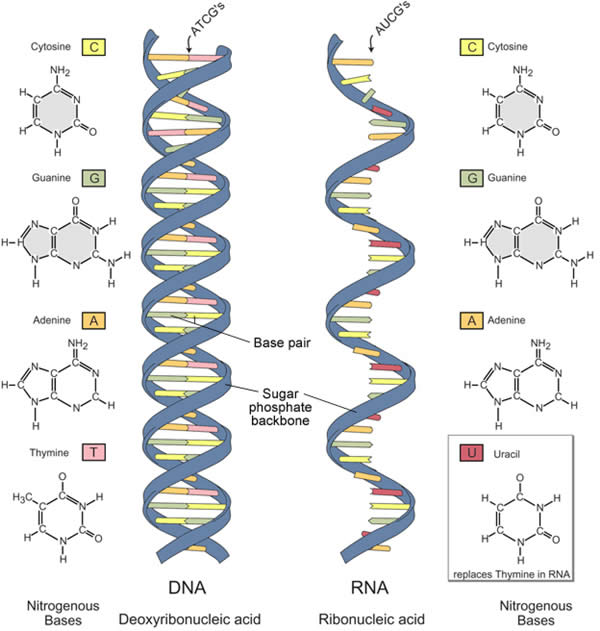
\includegraphics[width=\linewidth]{images/dna_rna.png}
  %\caption{C\'elulas Procariota y Eucariota.} 
  %\end{figure} 

  \subsubsection{C\'elulas}
  Son unidades b\'asicas que conforman el organismo y dentro de \'estas ocurren todas las funciones vitales. Adem\'as contienen la informaci\'on gen\'etica en su ADN, la cual se transmite a las c\'elulas hijas. Existen dos tipos:
  \begin{enumerate}
    \item \textit{Procariotas}: Carecen de membrana nuclear.
    \item \textit{Eucariotas}: Poseen un n\'ucleo bien definido mediante una membrana nuclear que contiene al ADN.
  \end{enumerate}

  \subsection{La Estructura Secundaria Del ARN}\label{estructuraSecundariaARN}
  El plegamiento de una secuencia de ARN entre sus bases complementarias determina lo que se denomina \emph{estructura secundaria de ARN}. Conocer la 
  estructura secundaria es fundamental para comprender el funcionamiento de los distintos tipos de ARN y de la c\'elula en general. Existen diferentes
  tipos de ARN, distingui\'endose entre ellos:
  \begin{itemize}
    \item \textit{Messenger ARN} (mRNA).
    \item \textit{Ribosomal ARN} (rRNA).
    \item \textit{Transfer ARN} (tRNA).
  \end{itemize}

  La existencia del t\'ermino \emph{estructura secundaria} nos hace suponer tambi\'en la existencia de una \emph{estructura primaria}. Como se mencion\'o, dicha estructura queda representada mediante una secuencia de nucle\'otidos. Tambi\'en existe la estructura terciaria de ARN, pero se la deja a un lado por no
  ser relevante en este trabajo.

  \begin{definition}
    \label{rna_primary}
    La estructura primaria del ARN, es una secuencia de nucle\'otidos de longitud
    $n$, $A=a_{1}a_{2}a_{3}\dots a_{n}$ con $a_{i} \in \left\lbrace A, U, G, C
    \right\rbrace$ 
  \end{definition}

  \begin{definition}
    \label{rna_secondary}
    Dada una estructura primaria o secuencia de RNA de longitud $n$, la
    estructura secundaria es un conjunto S de pares $(i,j)$ con $1\leq i < j \leq
    n$ tal que para todo, $(i,j), (i',j') \in S$ se satisfacen las tres siguientes
    condiciones:
    \begin{itemize}
      \item $j-i > 3$
      \item $i=i' \Leftrightarrow j=j'$
      \item $i< i'\Rightarrow i < i' < j' < j \lor i < j < i' < j'$ 
    \end{itemize}
  \end{definition}

  \subsection{Energ\'ia Libre y Estabilidad}
  El concepto de ``Energ\'ia Libre'' hace referencia a la energ\'ia total contenida en un sistema, como por ejemplo una mol\'ecula de ARN con una estructura secundaria, la cual le permite al mismo realizar trabajo. Una mol\'ecula de ARN puede estar dotada de una cierta cantidad de energ\'ia libre mediante interacciones el\'ectricas no neutralizadas en su estructura primaria, por lo tanto, esta energ\'ia se utilizar\'a para plegar la misma hacia una estructura secundaria m\'as estable. De este modo, un ARN con una estructura secundaria estable, implica una mol\'ecula en la cual sus interacciones el\'ectricas entre nucle\'otidos se hallan completamente neutralizadas. Se podr\'ia inferir que si una secuencia viral de ARN mutada tiene energ\'ia libre m\'inima, la misma no variar\'a su estructura secundaria por s\'i sola. 
  
  \subsection{Virus HIV}
  Los virus son entidades infecciosas microsc\'opicas que pueden multiplicarse dentro de las c\'elulas de un organismo dado. El virus HIV (\emph{Human immunodeficiency virus}) infecta a c\'elulas vitales del sistema inmunol\'ogico humano, tales como los \textit{Linfocitos T} (espec\'ificamente los que contienen receptores CD4$^+$), los \textit{macr\'ofagos} y las \textit{c\'elulas dendr\'iticas}. Las CD4$^+$ son un sub-grupo de los linfocitos, un tipo de gl\'obulos
  blancos, los cuales desempe\~nan un rol importante en el establecimiento y maximizaci\'on del sistema de defensa de un organismo.

  La infecci\'on con HIV lleva a un nivel bajo de c\'elulas T CD4$^+$. En el instante en que \'estas llegan a un nivel cr\'itico, se pierde la
  inmunidad celular y el organismo, progresivamente, se vuelve cada vez m\'as susceptible a otras infecciones oportunistas.

  \subsection{SIDA}
  El SIDA, del acr\'onimo \textbf{S}\'indrome de \textbf{I}nmunodeficiencia \textbf{A}dquirida, es una enfermedad que afecta a los humanos infectados
  por el HIV tipo 1. Se dice que una persona padece de SIDA cuando su organismo, debido a la inmunodeficiencia provocada por el HIV, no es capaz de ofrecer
  una respuesta inmune adecuada contra las infecciones.

  Cabe destacar la diferencia entre estar infectado por el HIV y padecer de SIDA. Una persona infectada por el HIV es \textit{seropositiva}\footnote{el
  t\'ermino seropositivo se aplica a una condici\'on inmunitaria, caracterizada por la presencia de un anticuerpo espec\'ifico en sangre, creado frente
  a un ant\'igeno que puede provenir de un agente infeccioso como de uno no infeccioso.} la cual luego desarrolla un cuadro de SIDA cuando su nivel de
  linfocitos T CD4$^+$ desciende por debajo de 200 c\'elulas por mililitro de sangre.

  \subsection{Antirretrovirales}
  Los f\'armacos utilizados en tratamientos actuales para combatir las infecciones con HIV son denominados antirretrovirales. Existe una variedad de estos
  provenientes de distintos laboratorios, cada uno con sus respectivas caracter\'isticas, los cuales se clasifican por su rango de acci\'on en dos clases: los \emph{Protease Inhibitors} (PI) y \emph{Reverse Transcriptase Inhibitors}. Dentro de la segunda clase hay dos sub-tipos que son los \emph{Nucleotide Reverse Transcriptase Inhibitors} (NRTI) y los \emph{Non-Nucleotide Reverse Transcriptase Inhibitors} (NNRTI). Existen otras dos clases m\'as recientes que son los \emph{Fusion or Entry Inhibitors} y los \emph{Integrase Inhibitors}. El objetivo de aplicar antirretrovirales a los pacientes es inhibir la replicaci\'on del virus por un tiempo indeterminado.

  A continuaci\'on se muestra una tabla conteniendo los antirretrovirales aprobados por la FDA (Food and Drugs Administration
  \url{http://www.fda.gov/MedicalDevices/default.htm}).


  M\'ultiples Clases Combinadas (Multi-class combinations):
  \begin{center}
    \begin{tabular}{|c|c|c|}
      \hline Combinaci\'on & Comercial & Aprobaci\'on \\ 
      \hline EFV + TDF + FTC & Atripia & 12-Jul-06 \\ 
      \hline d4T + 3TC + NVP & - & Tentative only* \\ 
      \hline AZT + 3TC+ NVP & - & Tentative only* \\ 
      \hline 
    \end{tabular}
  \end{center}

  Inhibidores de Transcriptasa Reversa Nucle\'osidos (NRTIs):

  \begin{center}
    \begin{tabular}{|c|c|c|c|}
      \hline Abreviaci\'on & Gen\'erico & Comercial & Aprobaci\'on \\ 
      \hline 3TC & lamivudine & Epivir & 17-Nov-95 \\ 
      \hline ABC & abacavir   & Ziagen & 17-Dec-98  \\ 
      \hline AZT o ZDV & zidovudine & Retrovir & 19-Mar-87 \\ 
      \hline d4T & stavudine & Zerit & 24-Jun-94  \\ 
      \hline ddI & didanosine & Videx EC & 31-Oct-00  \\ 
      \hline FTC & emtricitabine & Emtriva & 02-Jul-03 \\ 
      \hline TDF & tenofovir & Viread & 26-Oct-01  \\ 
      \hline 
    \end{tabular}
  \end{center}

  Inhibidores de Transcriptasa Reversa No Nucle\'osidos (NNRTIs):

  \begin{center}
    \begin{tabular}{|c|c|c|c|}
      \hline Abreviaci\'on & Gen\'erico & Comercial & Aprobaci\'on \\ 
      \hline DLV & delavirdine & - & 04-Apr-97 \\ 
      \hline EFV & efavirenz   & Sustiva & 17-Sep-98 \\ 
      \hline ETR & etravirine & Intelence & 18-Jan-08 \\ 
      \hline NVP & nevirapine & Viramune & 21-Jun-96 \\ 
      \hline 
    \end{tabular}
  \end{center}

  NRTIs Combinados (Combined NRTIs):

  \begin{center}
    \begin{tabular}{|c|c|c|}
      \hline Combinaci\'on & Comercial & Aprobaci\'on \\ 
      \hline ABC + 3TC & Epzicom (US) & 02-Aug-04  \\ 
      \hline ABC + AZT + 3TC & Trizivir & 14-Nov-00 \\ 
      \hline AZT + 3TC & Combivir & 27-Sep-97  \\ 
      \hline TDF + FTC & Truvada & 02-Aug-04  \\ 
      \hline d4T + 3TC & - & Tentative only*  \\ 
      \hline 
    \end{tabular}
  \end{center}

  Inhibidores de Proteasa (Protease Inhibitors) (PIs):

  \begin{center}
    \begin{tabular}{|c|c|c|c|}
      \hline Abreviaci\'on & Gen\'erico & Comercial & Aprobaci\'on \\
      \hline APV & amprenavir & Agenerase & 15-Apr-99  \\ 
      \hline FOS-APV & fosamprenavir & Lexiva (US) & 20-Oct-03 \\ 
      \hline ATV & atazanavir & Reyataz & 20-Jun-03 \\ 
      \hline DRV & darunavir & Prezista & 23-Jun-06 \\ 
      \hline IDV & indinavir & Crixivan & 13-Mar-96 \\ 
      \hline LPV/RTV & lopinavir + ritonavir & Kaletra & 15-Sep-00 \\ 
      \hline NFV & nelfinavir & Viracept & 14-Mar-97	 \\ 
      \hline RTV & ritonavir & Norvir & 01-Mar-96 \\ 
      \hline SQV & saquinavir & Invirase & 06-Dec-95 \\ 
      \hline TPV & tipranavir & Aptivus & 22-Jun-05 \\ 
      \hline 
    \end{tabular} 
  \end{center}

  Inhibidores de Fusi\'on o Entrada (Fusion or Entry Inhibitors):

  \begin{center}
    \begin{tabular}{|c|c|c|c|}
      \hline Abreviaci\'on & Gen\'erico & Comercial & Aprobaci\'on \\ 
      \hline T-20	& enfuvirtide &	Fuzeon & 13-Mar-03  \\ 
      \hline MVC & maraviroc &Celsentri & 18-Sep-07 \\ 
      \hline 
    \end{tabular}
  \end{center}

  Inhibidores de Integrasa (Integrase Inhibitors):

  \begin{center}
    \begin{tabular}{|c|c|c|c|}
      \hline Abreviacia\'on & Gen\'erico & Comercial & Aprobaci\'on \\ 
      \hline RAL & raltegravir & Isentress & 12-Oct-07  \\ 
      \hline 
    \end{tabular} 
  \end{center}

  \subsection{Fracaso, o Fallo, Terap\'eutico Para El HIV}\label{fracasoTerapeutico}
  El fracaso terap\'eutico, o de tratamiento, ocurre cuando los medicamentos para HIV no pueden controlar la infecci\'on de un modo eficiente.
  Existen tres tipos de fracaso terap\'eutico: \textbf{fallo virol\'ogico}, \textbf{fallo inmunol\'ogico} y \textbf{fallo cl\'inico}.

  El fracaso virol\'ogico ocurre cuando los antirretrovirales no pueden disminuir la carga viral en sangre. De este modo, aunque el paciente est\'e tomando los 
  medicamentos proscritos, la cantidad de virus en sangre no disminuye o bien se eleva repetidamente.

  El fracaso inmunol\'ogico ocurre cuando el sistema inmunitario no responde a los medicamentos antirretrovirales. De este modo, aunque tome los medicamentos, el recuento de linfocitos CD4+ no disminuye ni se incrementa.

  El fracaso cl\'inico se presenta cuando, a pesar que el paciente toma los medicamentos antirretrovirales, persisten los s\'intomas de infecci\'on por VIH.

  Los tres tipos de fracaso terap\'eutico pueden ocurrir solos o simult\'aneamente. Por lo general, primero ocurre el fracaso virol\'ogico, seguido por el
  fracaso inmunol\'ogico y luego se presenta el fracaso cl\'inico. Pueden ocurrir en un lapso de meses o a\~nos entre s\'i mismos.

  \subsubsection{?`Cu\'ales son los factores de riesgo para el fracaso terap\'eutico?}
  Los factores que pueden incrementar el riesgo del fracaso terap\'eutico incluyen:
  \begin{itemize}
    \item Fracaso terap\'eutico previo
    \item \textbf{Resistencia farmacol\'ogica} (o resistencia al medicamento)
    \item Falta de adherencia al tratamiento
    \item El organismo no absorbe debidamente los medicamentos antirretrovirales
    \item Cualquier otra enfermedad o afecci\'on
    \item Mala salud antes de comenzar el tratamiento
    \item Efectos secundarios de los medicamentos o interacciones con otros medicamentos
    \item Abuso de sustancias t\'oxicas que ocasionan falta de adherencia al tratamiento.
  \end{itemize}

  \subsection{Otros T\'erminos}
  \begin{description}
    \item \textbf{Adherencia al tratamiento:} consiste en seguir (acatar) cuidadosamente un r\'egimen de tratamiento. Eso incluye tomar la dosis correcta
      de un medicamento en el momento adecuado, exactamente como se lo recetaron.
    \item \textbf{Carga viral:} cantidad de HIV en una muestra de sangre. La carga viral mide qu\'e tan bien est\'an controlando la infecci\'on los
          antirretrovirales.
    \item \textbf{Pruebas de resistencia farmacol\'ogica:} pruebas de laboratorio para determinar si el VIH de una persona es resistente a cualquier
          medicamento antirretroviral.
    \item \textbf{Recuento de linfocitos CD4+:} Un recuento CD4+ es la cantidad de linfocitos CD4+ en una muestra de sangre. El recuento CD4+ mide la salud
      del sistema inmunitario.
    \item \textbf{Resistencia farmacol\'ogica:} El HIV puede mutar (EL ARN cambia su secuencia de nucle\'otidos para hacerse resistente a un antirretroviral). El VIH alterado se puede multiplicar incluso en presencia de medicamentos antirretrovirales que normalmente matar\'ian el virus. Uno o m\'as medicamentos en un r\'egimen de tratamiento pueden volverse ineficaces como resultado de la resistencia farmacol\'ogica.
    \item \textbf{Resistencia inmunol\'ogica:} Las nuevas pruebas no muestran aumento del recuento de linfocitos CD4+ a pesar del tratamiento. Un descenso en
      el recuento CD4+ mientras el paciente toma antirretrovirales puede indicar tambi\'en fracaso inmunol\'ogico.
  \end{description}

